% \documentclass[handout]{beamer}
\documentclass{beamer}

\mode<presentation>
{
  \usetheme{ANLBlue}
  % \usefonttheme[onlymath]{serif}
  % \usetheme{Singapore}
  % \usetheme{Warsaw}
  % \usetheme{Malmoe}
  % \useinnertheme{circles}
  % \useoutertheme{infolines}
  % \useinnertheme{rounded}

  \setbeamercovered{transparent=20}
}

\usepackage[english]{babel}
\usepackage[latin1]{inputenc}
\usepackage{alltt,listings,multirow,ulem,siunitx}
\usepackage[absolute,overlay]{textpos}
\TPGrid{1}{1}
\usepackage{pdfpages}
\usepackage{ulem}
\usepackage{multimedia}
\usepackage{multicol}
\newcommand\hmmax{0}
\newcommand\bmmax{0}
\usepackage{bm}
\usepackage{comment}
\usepackage{subcaption}

% font definitions, try \usepackage{ae} instead of the following
% three lines if you don't like this look
\usepackage{mathptmx}
\usepackage[scaled=.90]{helvet}
% \usepackage{courier}
\usepackage[T1]{fontenc}
\usepackage{tikz}
\usetikzlibrary{decorations.pathreplacing}
\usetikzlibrary{shadows,arrows,shapes.misc,shapes.arrows,shapes.multipart,arrows,decorations.pathmorphing,backgrounds,positioning,fit,petri,calc,shadows,chains,matrix}

\newcommand\vvec{\bm v}
\newcommand\bvec{\bm b}
\newcommand\bxk{\bvec_0 \times \kappa_0 \cdot \nabla}
\newcommand\delp{\nabla_\perp}

% \usepackage{pgfpages}
% \pgfpagesuselayout{4 on 1}[a4paper,landscape,border shrink=5mm]

% \usepackage{JedMacros}

\newcommand{\timeR}{t_{\mathrm{R}}}
\newcommand{\timeW}{t_{\mathrm{W}}}
\newcommand{\mglevel}{\ensuremath{\ell}}
\newcommand{\mglevelcp}{\ensuremath{\mglevel_{\mathrm{cp}}}}
\newcommand{\mglevelcoarse}{\ensuremath{\mglevel_{\mathrm{coarse}}}}
\newcommand{\mglevelfine}{\ensuremath{\mglevel_{\mathrm{fine}}}}

%solution and residual
\newcommand{\vx}{\ensuremath{x}}
\newcommand{\vc}{\ensuremath{\hat{x}}}
\newcommand{\vr}{\ensuremath{r}}
\newcommand{\vb}{\ensuremath{b}}

%operators
\newcommand{\vA}{\ensuremath{A}}
\newcommand{\vP}{\ensuremath{I_H^h}}
\newcommand{\vS}{\ensuremath{S}}
\newcommand{\vR}{\ensuremath{I_h^H}}
\newcommand{\vI}{\ensuremath{\hat I_h^H}}
\newcommand{\vV}{\ensuremath{\mathbf{V}}}
\newcommand{\vF}{\ensuremath{F}}
\newcommand{\vtau}{\ensuremath{\mathbf{\tau}}}


\title{Present and Future Computing Requirements for PETSc}
\author{{\bf Jed Brown} \texttt{jedbrown@mcs.anl.gov}}

% - Use the \inst command only if there are several affiliations.
% - Keep it simple, no one is interested in your street address.
\institute
{ \small
  Mathematics and Computer Science Division, Argonne National Laboratory \\
  {\small Department of Computer Science, University of Colorado Boulder}
}

\date{NERSC ASCR Requirements for 2017 \\ 2014-01-15}

% This is only inserted into the PDF information catalog. Can be left
% out.
\subject{Talks}


% If you have a file called "university-logo-filename.xxx", where xxx
% is a graphic format that can be processed by latex or pdflatex,
% resp., then you can add a logo as follows:

% \pgfdeclareimage[height=0.5cm]{university-logo}{university-logo-filename}
% \logo{\pgfuseimage{university-logo}}



% Delete this, if you do not want the table of contents to pop up at
% the beginning of each subsection:
% \AtBeginSubsection[]
% {
% \begin{frame}<beamer>
%   \frametitle{Outline}
%   \tableofcontents[currentsection,currentsubsection]
% \end{frame}
% }

% If you wish to uncover everything in a step-wise fashion, uncomment
% the following command:

% \beamerdefaultoverlayspecification{<+->}

\begin{document}
\lstset{language=C}
\normalem

\begin{frame}
  \titlepage
\end{frame}

\begin{frame}{Extending PETSc's Hierarchically Nested Solvers}
  \begin{description} \small
  \item[ANL] {\bf Lois C. McInnes}, {\bf Barry Smith}, Jed Brown, Satish Balay \\
  \item[UChicago] Matt Knepley
  \item[IIT] Hong Zhang
  \item[LBL] Mark Adams
  \end{description}
  \begin{itemize}
  \item Linear solvers, nonlinear solvers, time integrators, optimization methods (merged TAO)
  \item Maximize versatility and efficiency for existing and new applications
  \item Performance portability from laptops to Top 10 systems
  \item Algorithm R\&D for fundamental bottlenecks (e.g., memory bandwidth)
  \end{itemize}
\end{frame}

\begin{frame}{Library-oriented workflow}
  \begin{itemize}
  \item Partner with specific applications, but provide features to all
    \begin{itemize}
    \item Recognize commonality, simple and versatile abstractions, reusable implementation
    \item We don't know most of our users, avg 50 emails/day
    \item We hope to hear about problems (algorithmic/convergence, performance, portability).
      Respond quickly.
    \end{itemize}
  \item Erratic use of supercomputing
    \begin{itemize}
    \item New development on laptops, workstations, and small servers
    \item Need to test new algorithm or new implementation
    \item Validate our expected performance models, find bottlenecks
    \item User reports scalability problem and we need to reproduce
    \end{itemize}
  \item Very short duration jobs across a range of sizes
    \begin{itemize}
    \item Strong and weak scaling studies
    \item Large jobs rarely run for more than 10 minutes
    \item Small runs take longer for strong scaling (up to a couple hours)
    \item Debug our code, user code (occasionally), and system implementation (e.g., MPI)
    \item 1-2 million hours at NERSC and ALCF/OLCF
    \end{itemize}
  \end{itemize}
\end{frame}

\begin{frame}{Computational characteristics}
  \begin{itemize}
  \item Assembled sparse linear algebra
    \begin{itemize}
    \item Arithmetic Intensity $< 0.25$ flops/byte (cf.~hardware at 8 flops/byte)
    \item Comfortable abstraction
    \item Adaptive coarsening, problems with poor geometric/multilevel structure
    \item Research: find higher level structure (UQ, implicit Runge-Kutta)
    \item Research: matrix-free, nonlinear methods, exotic multigrid/ephemeral data
    \end{itemize}
  \item Communication
    \begin{itemize}
    \item Neighbor ``halo exchange'' (bounded number of neighbors)
    \item Long-range communication to coarse process sets
    \item Reductions (blocking and non-blocking) where mathematically necessary (orthogonality)
    \end{itemize}
  \end{itemize}
\end{frame}

\begin{frame}{Research exemplars}
 \begin{columns}
   \begin{column}{0.7\textwidth}
     \includegraphics[width=\textwidth]{figures/TensorVsAssembly}
   \end{column}
   \begin{column}{0.3\textwidth}
     \begin{block}{Implicit Runge-Kutta}
       \begin{gather*}
         G = I \otimes S + J \otimes I
       \end{gather*}
     \end{block}
   \end{column}
 \end{columns}
 \begin{figure}
  \centering
  \begin{subfigure}[b]{0.18\textwidth}
    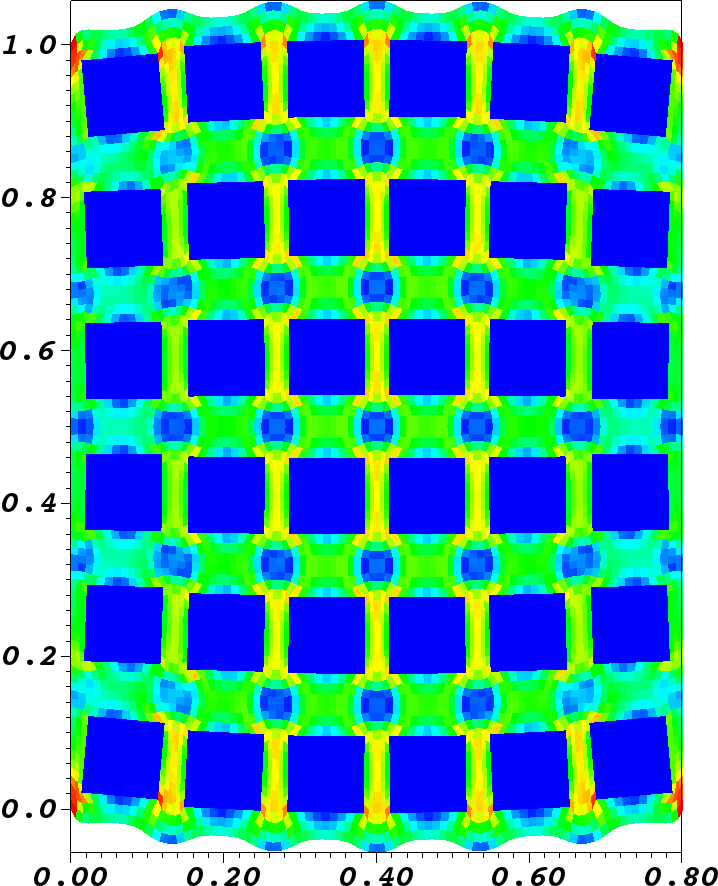
\includegraphics[width=\textwidth]{figures/MG/ElasticityCompressTrim}
    \caption{Initial solution.}\label{fig:elast-initial}
  \end{subfigure} ~
  \begin{subfigure}[b]{0.18\textwidth}
    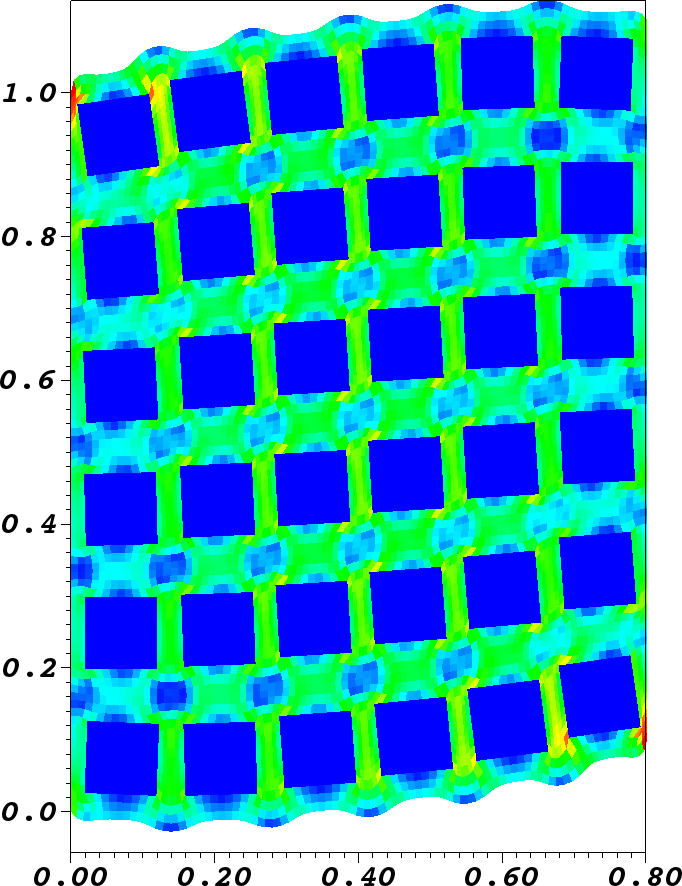
\includegraphics[width=\textwidth]{figures/MG/ElasticityCompressShearTrim}
    \caption{Increment.}\label{fig:elast-increment}
  \end{subfigure} ~
  \begin{subfigure}[b]{0.28\textwidth}
    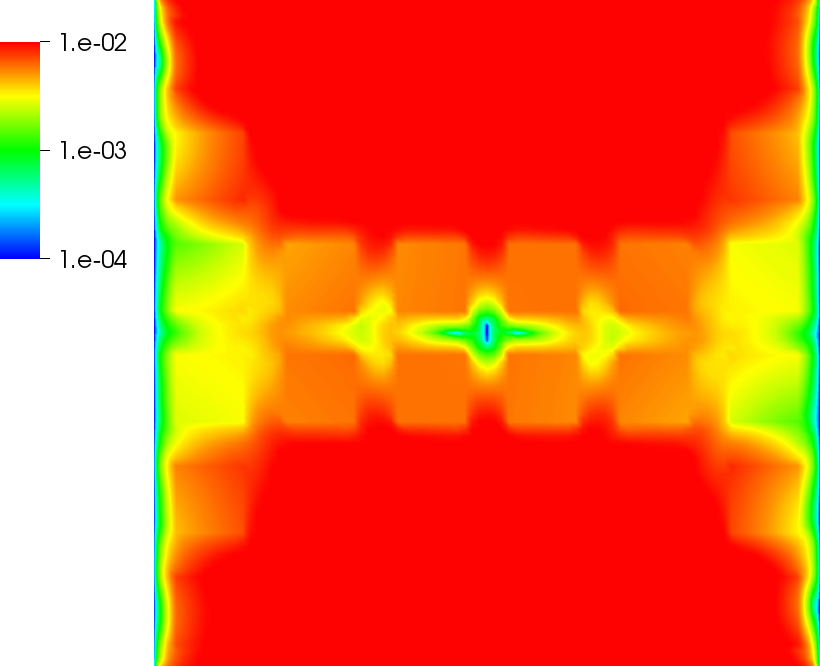
\includegraphics[width=\textwidth]{figures/MG/ElasticityCompressErrorNoTauTrim}
    \caption{Smoothed error without $\tau$.}\label{fig:elast-error-notau}
  \end{subfigure} ~
  \begin{subfigure}[b]{0.28\textwidth}
    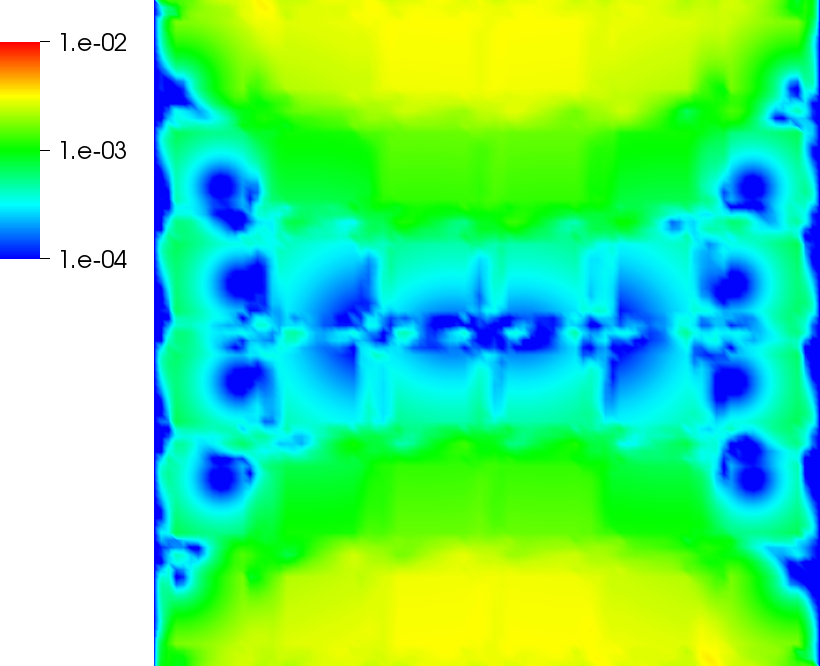
\includegraphics[width=\textwidth]{figures/MG/ElasticityCompressErrorTauTrim}
    \caption{Smoothed error with $\tau$.}\label{fig:elast-error-tau}
  \end{subfigure}
  % \caption{Plane strain elasticity with $E=1000,\nu=0.4$ inclusions in $E=1,\nu=0.2$ material, solved using 2-level multigrid with coarsening factor of $3^2$.
  %   The coarse (respectively fine) grid has 3 (9) $Q_1$ elements across each block and 2 (6) elements across each gap.
  %   Panes (a) and (b) show the deformed body colored by strain.
  %   The initial problem of compression by 0.2 from the right is solved (a) and $\tau = A^H \hat I_h^H u^h - I_h^H A^h u^h$ is computed.
  %   Then a shear increment of 0.1 in the $y$ direction is added to the boundary condition, and the coarse-level problem is resolved, interpolated to the fine-grid, and a post-smoother is applied.
  %   When the coarse problem is solved without a $\tau$ correction (c), the displacement error is nearly $10\times$ larger than when $\tau$ is included in the right hand side of the coarse problem (d).
  % }\label{fig:tau-valid}
  % ./ex49 -mx 90 -my 90 -da_refine_x 3 -da_refine_y 3 -elas_ksp_converged_reason -elas_ksp_rtol 1e-8 -no_view -c_str 3 -sponge_E0 1 -sponge_E1 1e3 -sponge_nu0 0.4 -sponge_nu1 0.2 -sponge_t 3 -sponge_w 9 -u_o vtk:ex49_sol.vts -use_nonsymbc -elas_pc_type mg -elas_pc_mg_levels 2 -elas_pc_mg_galerkin -tau1_o vtk:ex49_tau1.vts -tau2_o vtk:ex49_tau2.vts -taudiff_o vtk:ex49_taudiff.vts -u2_o vtk:ex49_sol2.vts -u2c_o vtk:ex49_sol2c.vts -u3_o vtk:ex49_sol3.vts -u4_o vtk:ex49_sol4.vts -u2err_o vtk:ex49_sol2err.vts -u3err_o vtk:ex49_sol3err.vts -u3c_o vtk:ex49_sol3c.vts -tau3_o vtk:ex49_tau3.vts
\end{figure}
\end{frame}

\begin{frame}{What is ``scalability''?}
  \begin{itemize}
  \item {\bf Transient simulation does not weak scale.}
    \begin{itemize}
    \item Fixed turn-around needed: policy, manufacturing/supply-chain, active control, real-time guidance (field work, surgery, etc.)
    \item $d$-dimensional problem, increase resolution by $2\times$.
    \item Data increases by $2^d$, but we need $2\times$ more time steps (hyperbolic).
    \item With perfect scaling, we use $2^{d+1}$ more cores.
    \item Local data changes by $2^d / 2^{d+1} = \frac 1 2$
    \end{itemize}
  \item More applications feeling this
    \begin{itemize}
    \item Asymptotics are relentless
    \item New analysis requires more solves in sequence
      \begin{itemize}
      \item From forward simulation to optimization with uncertainty \ldots
      \end{itemize}
    \item New physics and higher fidelity observation requires more calibration/validation
    \end{itemize}
  \item Other applications are safe for now
    \begin{itemize}
    \item Steady-state solves with scalable methods
    \item Transient with a small number of time steps
    \item Maximize resolution/problem size -- memory-constrained
    \end{itemize}
  \item<2> \alert{PETSc emphasizes \textbf{versatility}}
  \end{itemize}
\end{frame}

\begin{frame}{Indirect Challenges}
  \begin{itemize}
  \item Irresponsible library dependencies
    \begin{itemize}
    \item Difficult to install, non-portable, bad error-reporting
    \item Lack of 64-bit integers, \texttt{\_\_float128}
    \item Not scalable in $P$ (e.g., ParMETIS), assume non-empty subdomains
    \end{itemize}
  \item Misbehaving system software
    \begin{itemize}
    \item Broken features that we cannot test for
      \begin{itemize}
      \item \texttt{getpwuid} on BG/Q exists, but calling it rolls the
        dice between returning NULL, returning a valid pointer with
        junk, returning an invalid pointer, and crashing the program
        without returning.
      \item \texttt{MPI\_Bcast} and \texttt{MPI\_Comm\_split}
        deadlocking for large core count
      \item Users of various skill levels spend time tracking down
        issues and talking to us.
      \end{itemize}
    \item Useless performance and fragile run-time configuration
      \begin{itemize}
      \item No asynchronous progress for \texttt{MPI\_Iallreduce} in MPT-5.6+
      \item \texttt{MPICH\_ASYNC\_PROGRESS} helps a little (few percent)
      \item Affinity for async progress thread
      \end{itemize}
    \end{itemize}
  \item User knowledge and discipline
    \begin{itemize}
    \item Module environment changes between configure and make
    \item Portability limited by poorly-written code or build system
    \item Don't know about the barbed wire and broken glass
    \end{itemize}
  \end{itemize}
\end{frame}

\begin{frame}[shrink=5]{Strategies for New Architectures}
  \begin{itemize}
  \item Choose the right tool for the job.
  \item Typical GPU users are the least competent and have the least realistic expectations
  \item CUDA (CUSP \& CUSPARSE) and OpenCL (ViennaCL) Mat \& Vec
  \item Problem for matrix and vector assembly
    \begin{itemize}
    \item Bad abstractions for calling from thread block.  New kernel
      launches imply moving bulky intermediate to global memory.
    \end{itemize}
  \item User must write GPU code if they wish to have nonlinear
    residuals and matrix assembly use GPUs (Amdahl)
  \item Coupling apps/libs with different threading (OpenMP, TBB, pthreads)
  \item Defer choice of threading model to run-time (threadcomm)
  \item Less consistent performance, fragile run-time configuration
  \item Recommend MPI-only for most users
  \item Intel MIC is an abject failure of hardware and software.  Less
    efficient than Xeon for dense QR (all sizes), advertise useless
    OpenCL stack.  Maybe the next generation will be acceptable.
  \end{itemize}
\end{frame}

\begin{frame}{Some unpopular opinions}
  \begin{itemize}
  \item DSL --- informally-specified language with immature compiler
    \begin{itemize}
    \item Syntax or \emph{semantics}?
    \item Ability to use legacy (mature) code?  Debuggability?
    \end{itemize}
  \item Where is the fundamental complexity?
    \begin{itemize}
    \item Math and CS researchers often self-select a distorted perspective
    \item For long-term success, most code is written by domain scientists
    \item Material models, MD force models, ML feature extraction
    \item ``Kernels'' can have sprawling dependencies and $> 100 kLOC$
    \item Legacy and new experiments, written by non-experts
    \end{itemize}
  \item Granularity, static versus dynamic, versatility
    \begin{itemize}
    \item Small subdomains: surface area big compared to volume
    \item Over-decomposition lengthens the critical path
    \item We hear about $32^3$ patches/subdomains
      \begin{itemize}
      \item How efficient is one $8^3$ patch/node? $4^6$? 100 fields/cell?
      \end{itemize}
    \item Frequency of performance variation compared to latency to redistribute or steal
    \item Period of interruption/OS jitter
    \item Time between algorithmically-required data dependency?
    \end{itemize}
  % \item Global storage is dead as an algorithmic device
  \end{itemize}
\end{frame}

\begin{frame}{Summary}
  \begin{itemize}
  \item New algorithmic modifications become useful (scaling and hardware balance)
    \begin{itemize}
    \item Exotic low-communication multigrid
    \item Nonlinear and matrix-free methods
    \item Tensor product solvers (implicit Runge-Kutta, stochastic Galerkin)
    \item Efficient solver support for new discretizations
    \end{itemize}
  \item PETSc runs at NERSC need to keep pace with diverse user group
  \item Recommendations
    \begin{itemize}
    \item Emphasize versatility
    \item Identify ``cooked'' performance experiments
      \begin{itemize}
      \item Unrealistic problem sizes/turn-around time
      \item Artifical configurations
      \item Normalize by energy efficiency/acquisition cost/TCO, not shrink-wrap
      \end{itemize}
    \item Performance reproducibility, diagnostics, debugging
    \item Complicated execution environments will require a lot of
      education and a lot of support by third parties.
    \end{itemize}
  \end{itemize}
\end{frame}

\end{document}
